\section{Case Study}

\begin{frame}[fragile,allowframebreaks]{Open Source Projects}
    
\begin{figure}
    \centering
    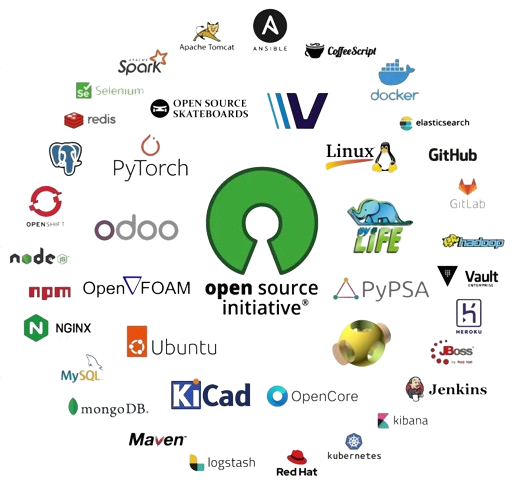
\includegraphics[width=0.42\linewidth]{assets/signal-2024-03-12-131914_002.png}
    % \caption{Open Source Projects}
    % \label{fig:enter-label}
\end{figure}

\end{frame}

\begin{frame}[fragile,allowframebreaks]{Enterprise Resource Planning Systems}
    
\begin{figure}
    \centering
    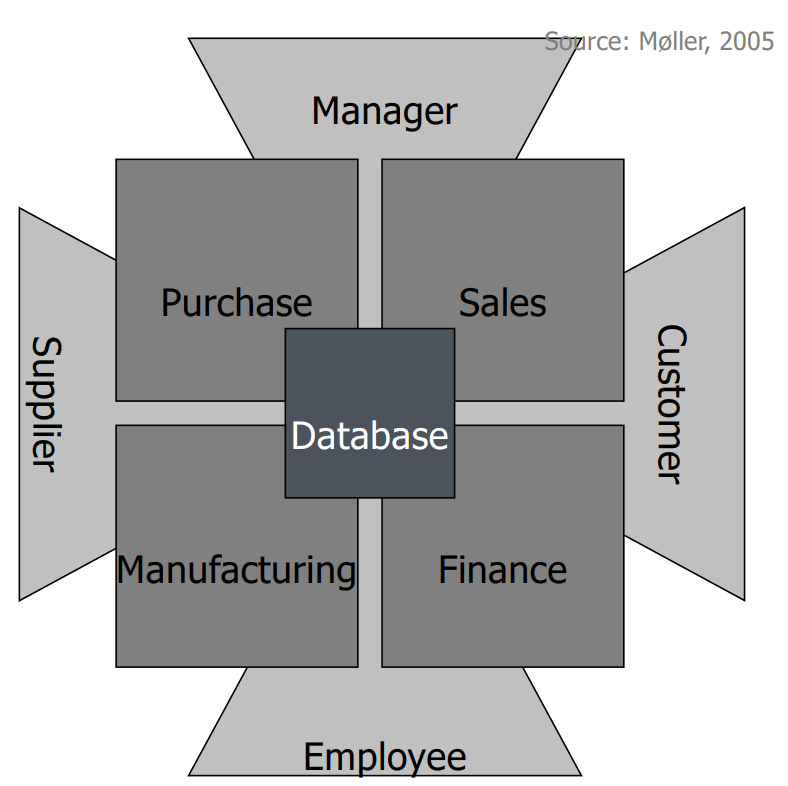
\includegraphics[width=0.40\linewidth]{assets/ERP.png}
    % \caption{Open Source Projects}
    % \label{fig:enter-label}
\end{figure}

\end{frame}

\begin{frame}[fragile,allowframebreaks]{SAP}
    
\begin{figure}
    \centering
    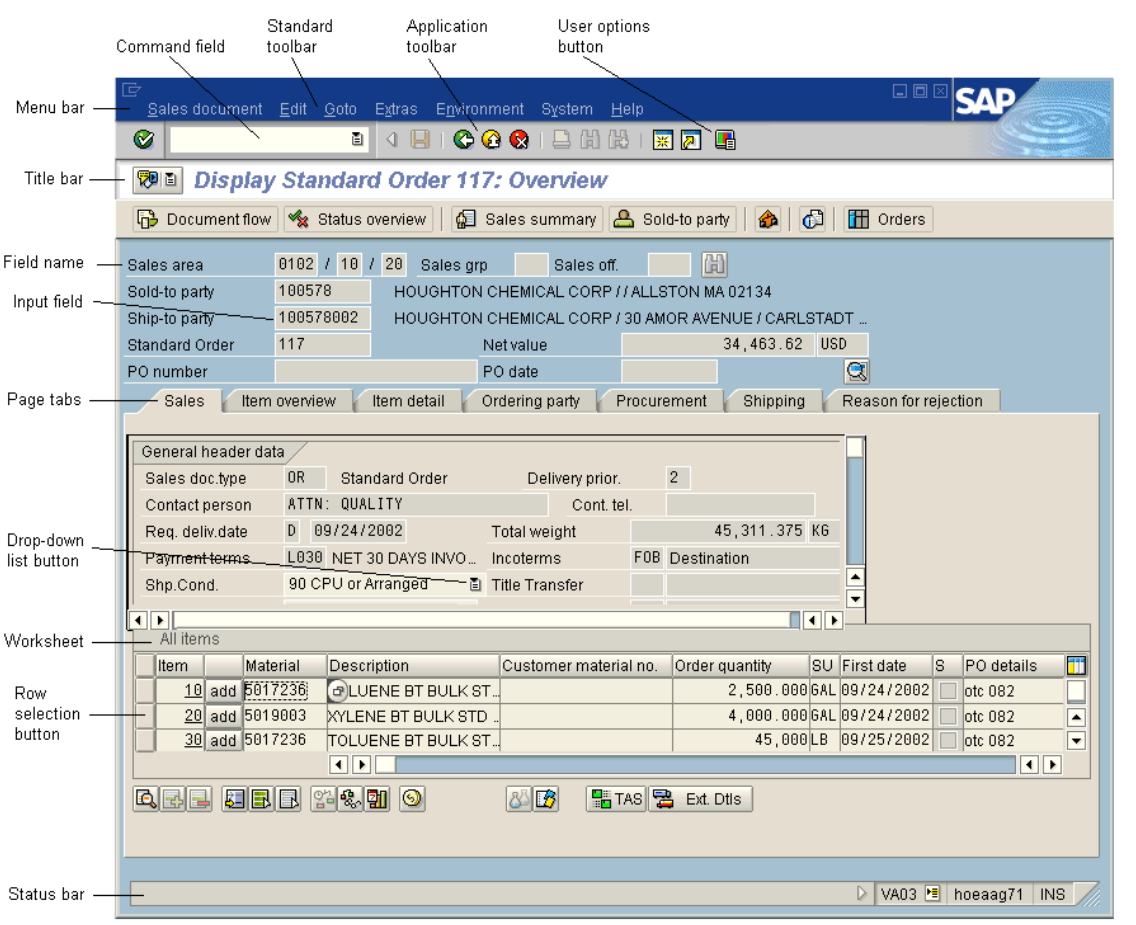
\includegraphics[width=0.50\linewidth]{assets/SAP.png}
    % \caption{Open Source Projects}
    % \label{fig:enter-label}
\end{figure}

\end{frame}
\begin{frame}[fragile,allowframebreaks]{Odoo}
    
\begin{figure}
    \centering
    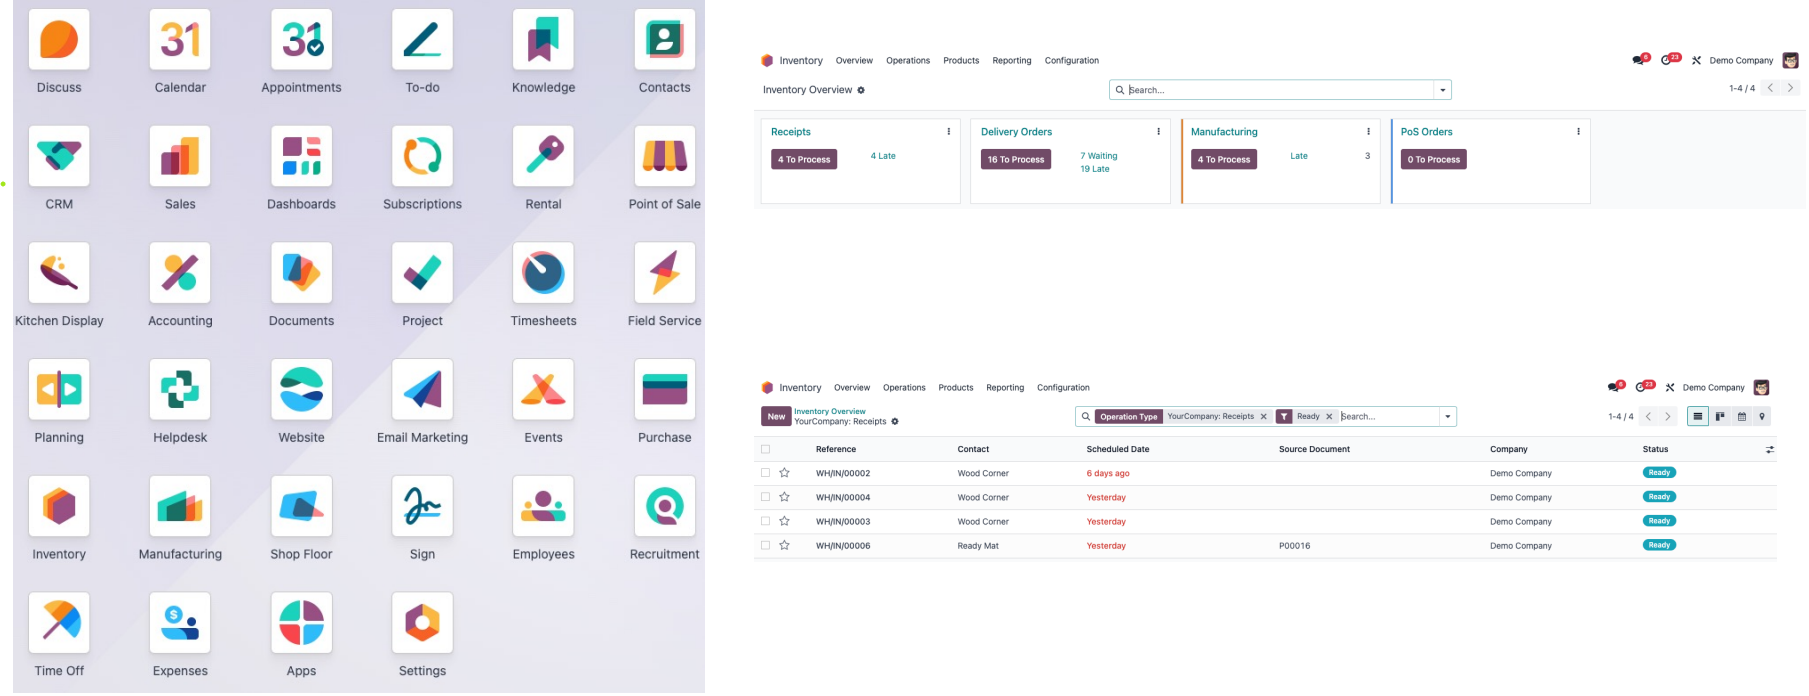
\includegraphics[width=0.90\linewidth]{assets/OdooInterface.png}
    % \caption{Open Source Projects}
    % \label{fig:enter-label}
\end{figure}

\end{frame}

\begin{frame}[fragile,allowframebreaks]{Odoo Pros and cons}
    \begin{table}[]
        \small
        \centering
        \def\arraystretch{1.1}
        \begin{tabular}{|c|c|}
        \hline
          \cellcolor{green!50}\textbf{Pros} & \cellcolor{red!50}\textbf{Cons} \\
        \hline
            $\blacktriangleright$ Transparency & $\blacktriangleright$ Lack of Support \\
            $\blacktriangleright$ Community collaboration & $\blacktriangleright$ Fragmentation \\
            $\blacktriangleright$ Customization & \color{gray}Perceived Lack of Accountability \\
            $\blacktriangleright$ Cost-Effective & \\
            $\blacktriangleright$ Innovation and rapid development & \\
            $\blacktriangleright$ Vendor Independence & \\
            $\blacktriangleright$ Learning Opportunities & \\

        \hline
        \end{tabular}
        % \caption{Pros and Cons}
        % \label{tab:ProsCons}
    \end{table}
    
\end{frame}

\begin{frame}[fragile,allowframebreaks]{Price Comparison}
    
\begin{figure}
    \centering
    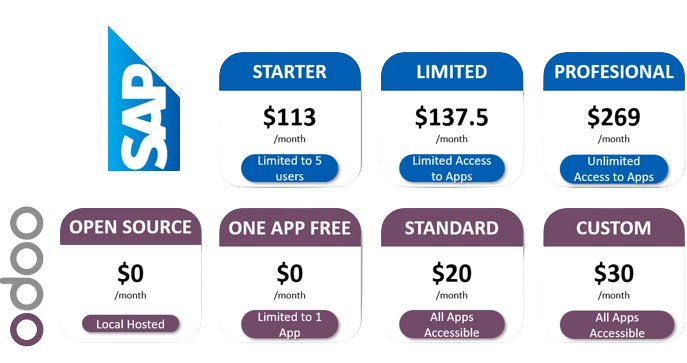
\includegraphics[width=0.70\linewidth]{assets/OdooPrices-removebg-preview.png}
    % \caption{Open Source Projects}
    % \label{fig:enter-label}
\end{figure}
\end{frame}

\begin{frame}[fragile,allowframebreaks]{What is TensorFlow? (I)}
    \begin{columns}[T]
        \column{0.99\textwidth}
            \vspace{1cm}
            \begin{itemize}
                \item Platform for machine learning
                \begin{itemize}
                    \item Machine learning library
                \end{itemize}
                \item Free and open source
                \begin{itemize}
                    \item License: Apache license 2.0
                    \item Initially from Google
                \end{itemize}
            \end{itemize}
        
         \column{0.01\textwidth}
             \vspace{-.1cm}
             \hspace*{-6cm}
             
\includegraphics[width=6cm]{assets/TensorFlow_logo_tp.png}
    \end{columns}
\end{frame}

\begin{frame}[fragile,allowframebreaks]{What is TensorFlow? (II)}
    \begin{columns}[T]
        \column{0.99\textwidth}
            \vspace{1cm}
                \begin{itemize}
                    \item Data flow graphs
                    \begin{itemize}
                        \item ML algorithms as a graph of connected operations
                        \item Quick and intuitive work flow
                    \end{itemize}
                \item Works with Python, C++ etc.
                \item Visualization of work by TensorBoard
                \end{itemize}
            \begin{figure}
                %\centering
                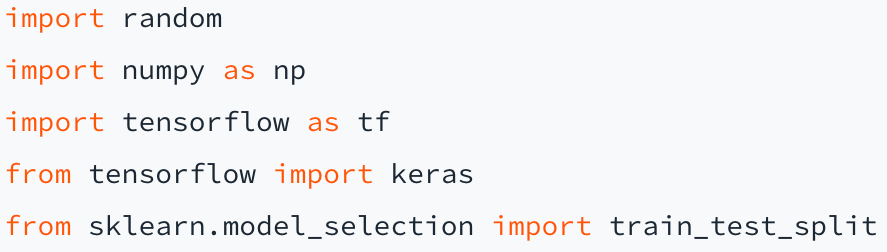
\includegraphics[width=0.50\linewidth]{assets/TensorFlow_Python.png}
                \\
                \source{Source: Udacity, Inc.}
                %\label{fig:enter-label}
            \end{figure}
         \column{0.01\textwidth}
            \vspace{.5cm}
            \hspace*{-4cm}
            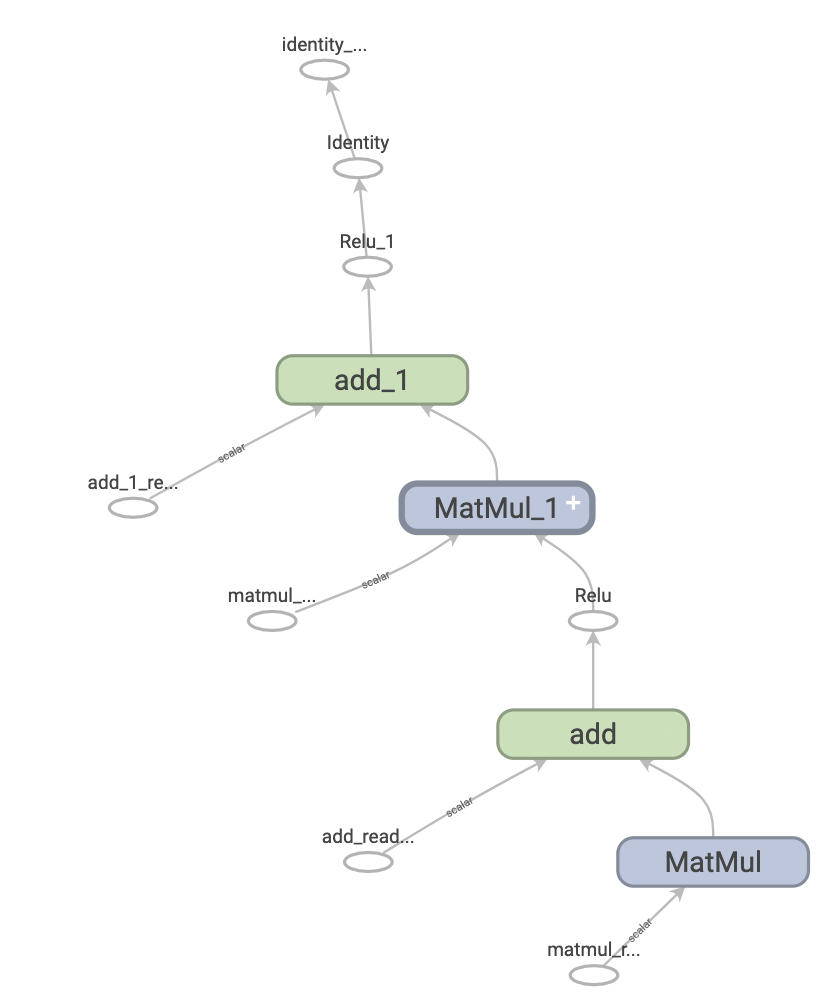
\includegraphics[width=4cm]{assets/TensorFlow_Graph_Example.png} 
                \\
                \vspace{-.1cm}
                \hspace*{-4cm}\caption{Source: tensorflow.org}
    \end{columns}
\end{frame}

\begin{frame}[fragile,allowframebreaks]{What is TensorFlow? (III)}
        \begin{columns}[T]
        \column{0.99\textwidth}
            \vspace{1cm}
            \begin{itemize}
                \item Natural language processing
                \item Image recognition
                \item Computational-based simulations
                \item Training and execution on GPUs, CPUs or TPUs (Cloud)
            \end{itemize}
        
         \column{0.01\textwidth}
             \vspace{-0cm}
             \hspace*{-5cm}
             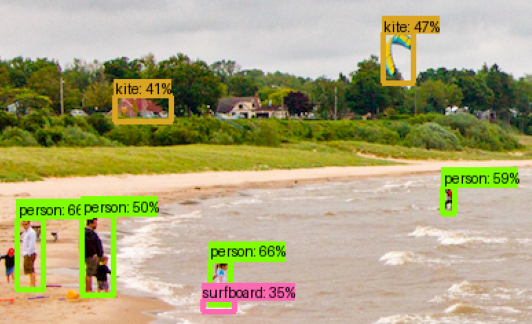
\includegraphics[width=5cm]{assets/TensorFlow_ObjectDetection(2).png}
                 \\
                 \vspace{-.1cm}
                 \hspace*{-5cm}\caption{Source: tensorflow.org}
        \end{columns}
\end{frame}

\begin{frame}[fragile,allowframebreaks]{Tensor flow: Open-source characteristics}
    \begin{itemize}
        \item Google as contributor \textbf{and} promoter
        \begin{itemize}
        \item Part of Googles business model
        \end{itemize}
        \item Network of collaborators 
        \item Beyond source code: Sharing of models and datasets
    \end{itemize}
\end{frame}

\begin{frame}[fragile,allowframebreaks]{Tensor flow: Google's perspective}
        \begin{columns}[T]
        \column{0.99\textwidth}
            \vspace{1cm}
        \begin{itemize}
            \item Google developed closed code until 2015
            \item Googles AI products use TensorFlow
            \item (Worldwide) collaboration - exposure
            \item More users, potential profit
            \begin{itemize}
                \item Googles cloud-TPUs
            \end{itemize}
        \end{itemize}
        
         \column{0.01\textwidth}
             \vspace{-0cm}
             \hspace*{-5cm}
             
\includegraphics[width=5cm]{assets/GoogleTransp.png}
                 \\
                 \vspace{-.1cm}
                 \hspace*{-5cm}
                 %\caption{Source: google.com}
        \end{columns}

\end{frame}

% \begin{frame}[fragile,allowframebreaks]{Tensor flow: Pros and cons}
%     \begin{itemize}
%         \item Well-documented
%         \item Widely used
%         \item Shared Datasets and ML models
%         \item Freedom to use and modify
%         \item Integration in business model
%         \item ???Cons???
%     \end{itemize}
% \end{frame}

\begin{frame}[fragile,allowframebreaks]{Tensor flow: Pros and cons}
    \begin{table}[]
        \small
        \centering
        \def\arraystretch{1.1}
        \begin{tabular}{|c|c|}
        \hline
          \cellcolor{green!50}\textbf{Pros} & \cellcolor{red!50}\textbf{Cons} \\
        \hline
            \color{gray}Transparency & \color{gray}Lack of Support \\
            $\blacktriangleright$ Community collaboration & \color{gray}Fragmentation \\
            \color{gray} Customization & \color{gray}Perceived Lack of Accountability \\
            \color{gray} Cost-Effective & \\
            $\blacktriangleright$ Innovation and rapid development & \\
            \color{gray}Vendor Independence & \\
            $\blacktriangleright$ Learning Opportunities & \\
            $\blacktriangleright$ Ethical Considerations & \\
            $\blacktriangleright$ \textit{Google as big contributor} & $\blacktriangleright$ \textit{Google as big contributor} \\
        \hline
        \end{tabular}
        % \caption{Pros and Cons}
        % \label{tab:ProsCons}
    \end{table}
\end{frame}